% Activate the following line by filling in the right side. If for example the name of the root file is Main.tex, write
% "...root = Main.tex" if the chapter file is in the same directory, and "...root = ../Main.tex" if the chapter is in a subdirectory.
 
%!TEX root = testMain.tex

\chapter[Introduction]{Introduction}

Reasoning with evidence in law is cool!




\textbf{The main research question for this Master's Thesis is: can we automatically create good Bayesian Networks that reflect the ground truth of simulations? If so, can we use this simulation + Bayesian Network setup to investigate BN idioms and methods for law more generally, to see how well the probabilistic approach holds up?}



\section{The problem with evidence}

When we find evidence for a hypothesis that we have held in the back of our minds, we then find the hypothesis more likely. 
This is the basic idea behind reasoning with evidence. In a constellation of hypotheses and pieces of evidence, we want
to construct a network that will lead us to believe as many true hypotheses as possible, given the evidence that we have.

However, evidence itself is elusive, and it's connection to hypotheses is as well - how can we be sure that some evidence supports
some hypothesis, and even if we know that it does, how can we express how strong the piece of evidence is? Some evidence
is very weak, and only after a tedious process of ruling out other factors and careful investigation and collection of other pieces
of evidence, we can come to a conclusion about a hypothesis. On the other hand, some evidence is so strong that it leaves no room for doubt.

We all have intuitions about evidence strength - but can we make these intuitions precise? Additionally, can we manage the complex
realities of weak evidence for many different hypotheses? 

\section{Bayes}

When we reason probabilistically with evidence, we want to use the gold standard - Bayes Law.
Let's say that we find some piece of evidence $e$, we want to know how our finding $e$ affects our belief in some hypothesis $h$. We can express how much we believe $h$ given $e$, using Bayes Law:

\[ P(h | e) =  \frac{P(e | h) \cdot P(h)}{P(e)}\]


This is the simplest form of Bayesian reasoning, one piece of evidence, and one hypothesis. But real life is not so simple, and we are constantly reasoning with many pieces of evidence, and `small' hypotheses can serve as stepping stones to greater hypotheses! One way of handling the complexity of interacting pieces of evidence and hypotheses is by using Bayesian Networks.

A Bayesian Network is a directed, acyclic graph that represents the joint probability distribution over a set of events \citep{pearl1988}. BNs have nodes and arcs. Formally, the nodes are random variables that represent events, in case of our Bayesian Networks, these nodes represent hypotheses and pieces of evidence. An arc represent a conditional relationships between two nodes. An example of a Bayesian Network can be seen in Figure~\ref{exampleBN}. The conditional probability is expressed in the conditional probability table (cpt) of every node. A node that is not conditionally dependent on any other node (has no incoming arcs) is independent. In the figure, this is the node `train\_on\_time\_in\_groningen'. Nodes with one or more incoming arcs are conditionally dependent on their parent node(s) (the node `station\_renovation\_zwolle'). The links between the nodes are links of conditional probability, and do not correspond to real-world causality, although they are sometimes interpreted as being causal \citep{Dawid2008}.

\begin{figure}[h]
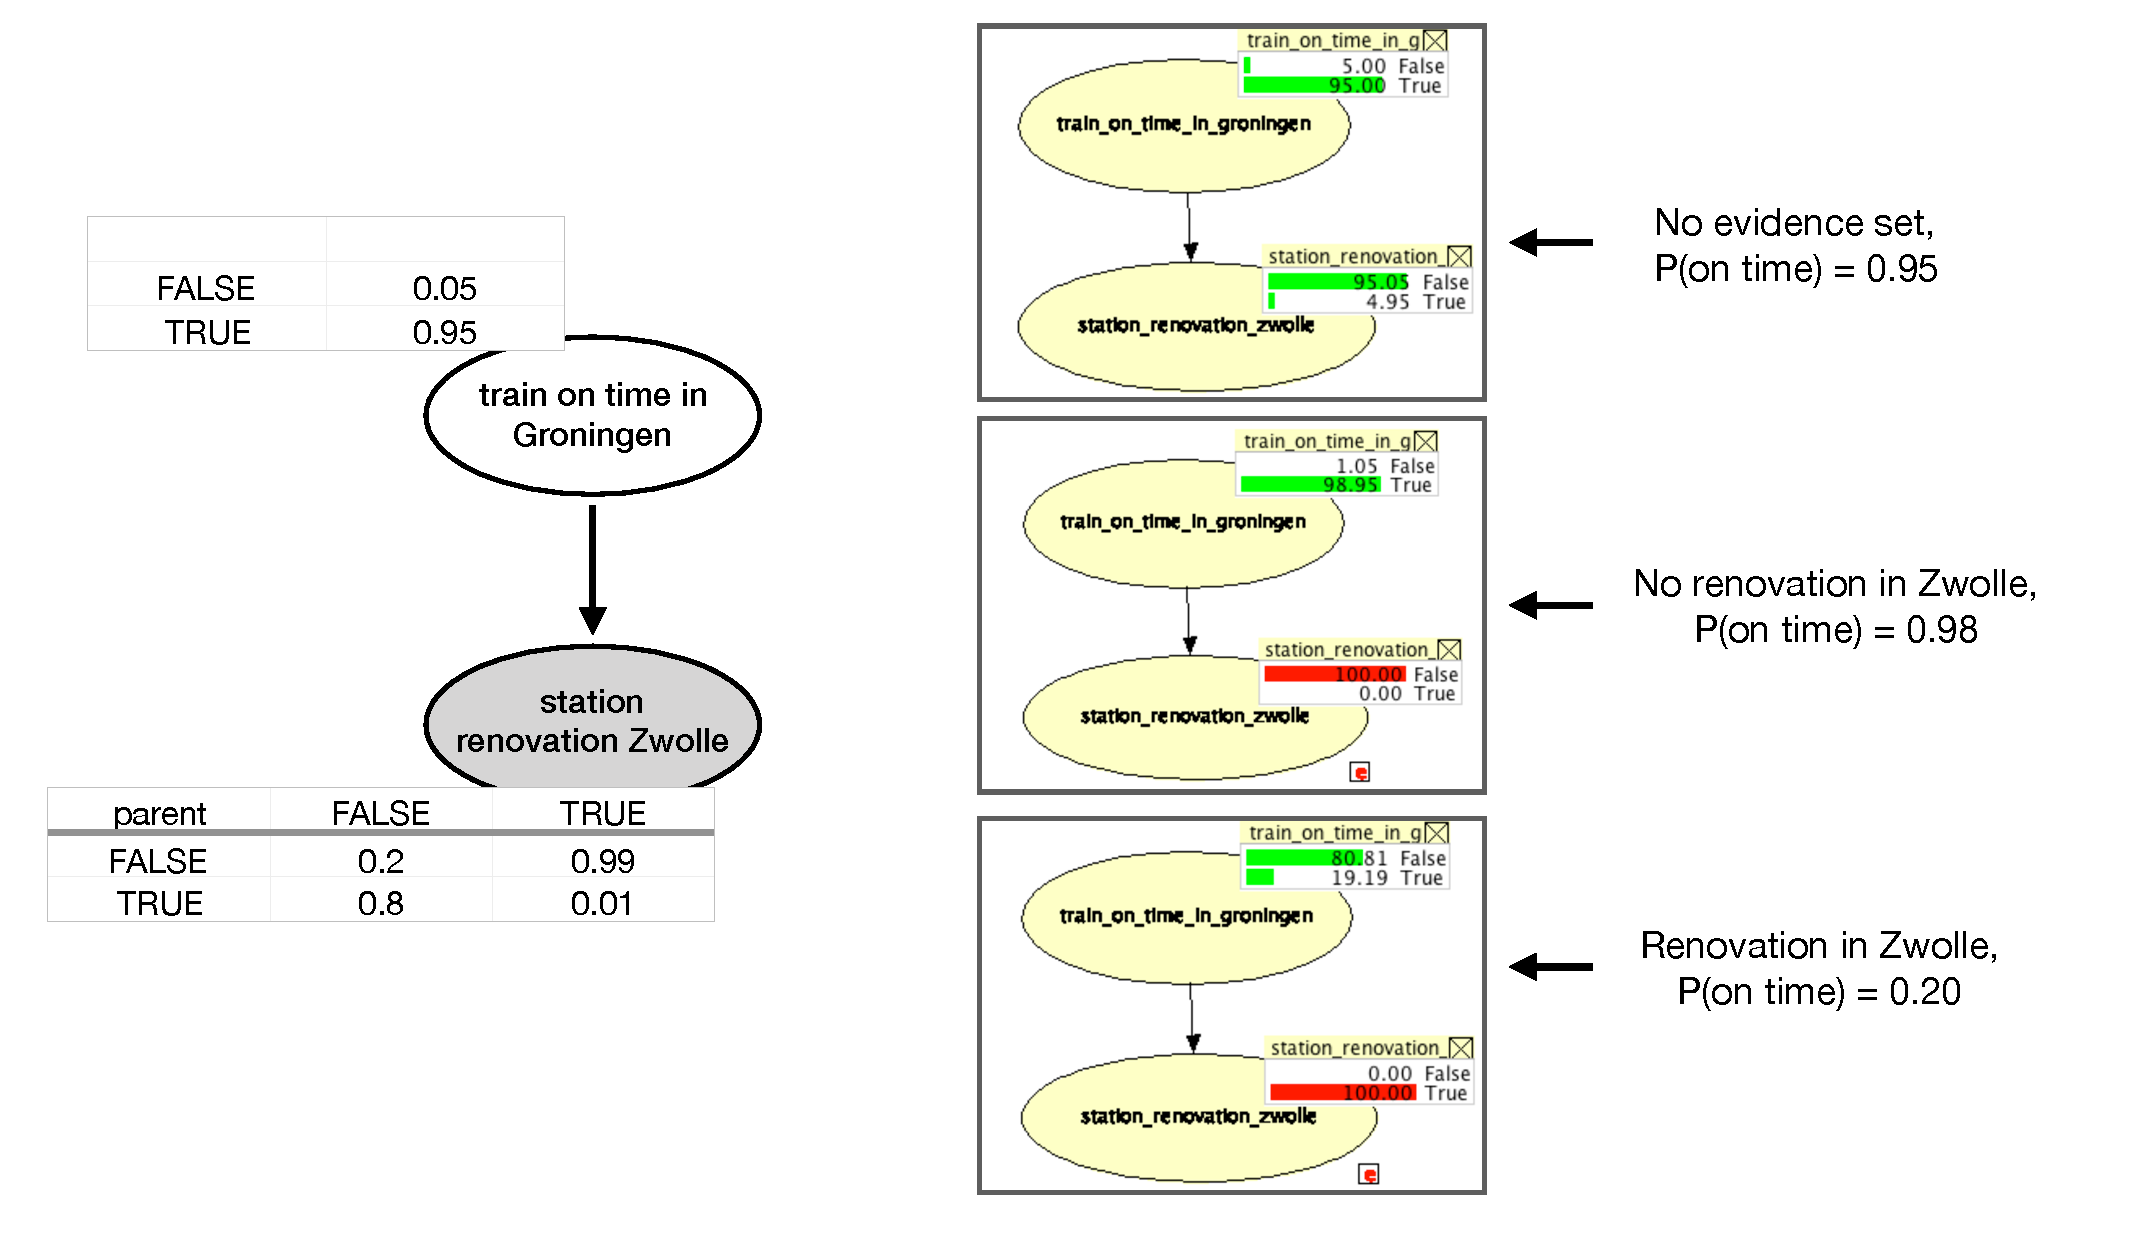
\includegraphics[width=\linewidth]{images/bnExample.pdf}
\label{exampleBN}
\caption{An example of a Bayesian Network, with and without evidence set.}
\end{figure}

We can reason with Bayesian Networks by setting evidence on one or more nodes that we can observe. This means that we say whether some observable node is true or false, and use that information to update the network. We can now find a new posterior probability for a node that we cannot observe directly (yet). In Figure~\ref{exampleBN}, this means that when there are station renovations going on at Zwolle, the probability that your train will be late in Groningen increases from a probability of 0.01, to a probability of 0.8.

\section{The New Idea of the Thesis}
We want to ground our Bayesian crime situations in multi-agent systems, so that we can have total control over whatever is happening, and we collect exactly the frequency information that we need.

Research Questions:


\section{Overview of the thesis}
Chapter 2 represents an overview of the state of the art, Chapter 3 proposes a pipeline for creating simulations and automatic Bayesian Networks, and evaluation criteria. Chapter 4, 5 and 6 are applications of this pipeline in three separate simulations: first a simple, non-spatial simulation based on \citep{Vlek2015}, a simple spatial simulation of a home-robbery, and finally a spatial simulation of a street-robbery. For each of these simulations, some simple experiments are done to investigate several problematic aspects of Bayesian Networks. These simulations are then each evaluated based on the evaluation criteria set out in Chapter 3. Finally, we draw conclusions in Chapter 7. 

You can interact with the simulation in Chapter 6 on \url{https://shielded-journey-34533.herokuapp.com}.

Code for this project can be found at \url{https://github.com/aludi/simulationTest}.
